% Created by tikzDevice version 0.12.3.1 on 2022-09-01 15:48:06
% !TEX encoding = UTF-8 Unicode
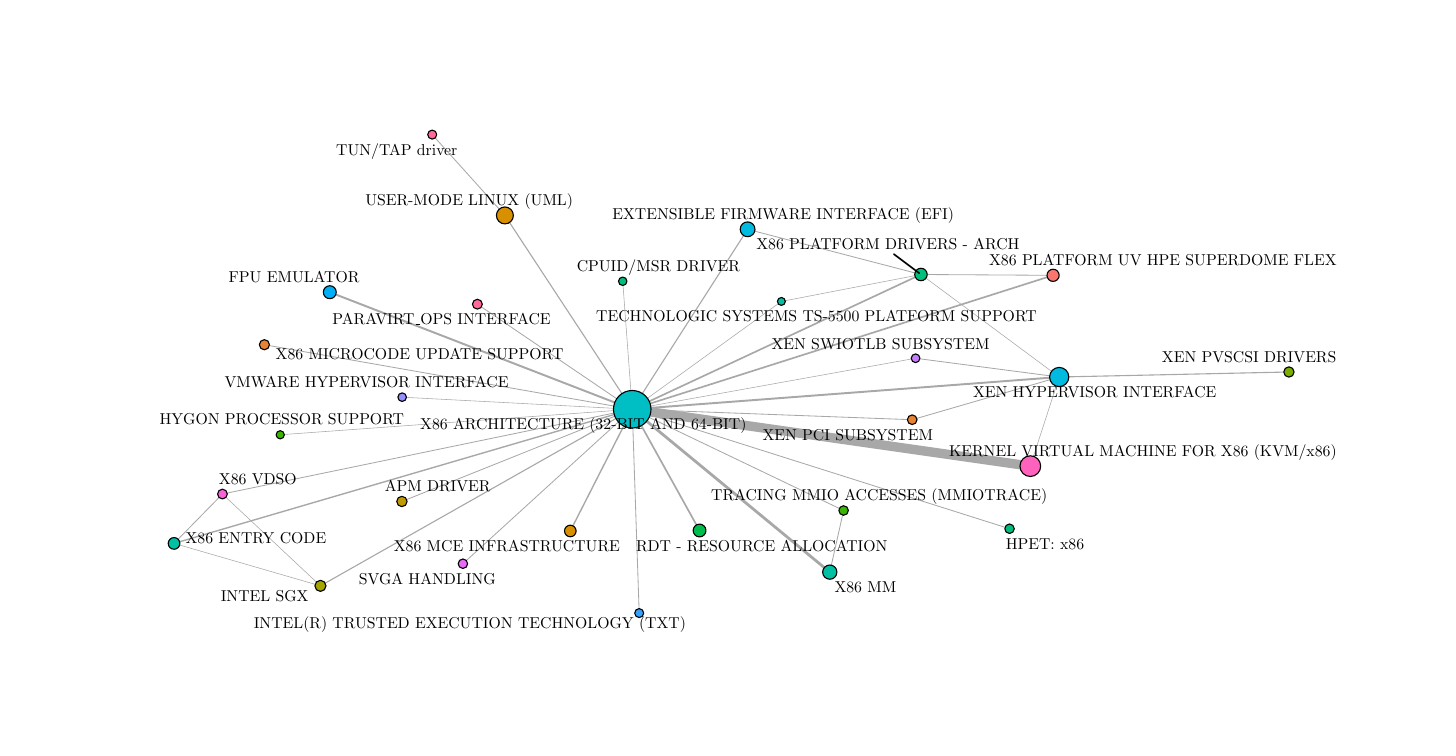
\begin{tikzpicture}[x=1pt,y=1pt]
\definecolor{fillColor}{RGB}{255,255,255}
\path[use as bounding box,fill=fillColor,fill opacity=0.00] (0,0) rectangle (505.89,252.94);
\begin{scope}
\path[clip] (  0.00,  0.00) rectangle (505.89,252.94);
\definecolor{fillColor}{RGB}{255,255,255}

\path[fill=fillColor] (  0.00,  0.00) rectangle (505.89,252.94);
\end{scope}
\begin{scope}
\path[clip] ( 32.75, 32.75) rectangle (475.89,222.94);
\definecolor{drawColor}{gray}{0.66}

\path[draw=drawColor,line width= 0.3pt,line join=round] (135.23, 81.73) -- (218.46,115.05);

\path[draw=drawColor,line width= 0.2pt,line join=round] (215.02,161.30) -- (218.46,115.05);

\path[draw=drawColor,line width= 0.4pt,line join=round] (260.14,180.08) -- (218.46,115.05);

\path[draw=drawColor,line width= 0.3pt,line join=round] (260.14,180.08) -- (322.79,163.75);

\path[draw=drawColor,line width= 0.7pt,line join=round] (109.17,157.35) -- (218.46,115.05);

\path[draw=drawColor,line width= 0.3pt,line join=round] (354.79, 71.88) -- (218.46,115.05);

\path[draw=drawColor,line width= 0.2pt,line join=round] ( 91.26,105.83) -- (218.46,115.05);

\path[draw=drawColor,line width= 0.4pt,line join=round] (105.79, 51.24) -- (218.46,115.05);

\path[draw=drawColor,line width= 0.2pt,line join=round] (105.79, 51.24) -- ( 52.89, 66.58);

\path[draw=drawColor,line width= 0.2pt,line join=round] (105.79, 51.24) -- ( 70.38, 84.42);

\path[draw=drawColor,line width= 0.3pt,line join=round] (220.97, 41.40) -- (218.46,115.05);

\path[draw=drawColor,line width= 3.4pt,line join=round] (362.30, 94.50) -- (218.46,115.05);

\path[draw=drawColor,line width= 0.2pt,line join=round] (362.30, 94.50) -- (372.74,126.70);

\path[draw=drawColor,line width= 0.3pt,line join=round] (162.50,153.02) -- (218.46,115.05);

\path[draw=drawColor,line width= 0.6pt,line join=round] (242.78, 71.24) -- (218.46,115.05);

\path[draw=drawColor,line width= 0.3pt,line join=round] (157.27, 59.24) -- (218.46,115.05);

\path[draw=drawColor,line width= 0.2pt,line join=round] (272.35,154.01) -- (218.46,115.05);

\path[draw=drawColor,line width= 0.2pt,line join=round] (272.35,154.01) -- (322.79,163.75);

\path[draw=drawColor,line width= 0.3pt,line join=round] (294.83, 78.47) -- (218.46,115.05);

\path[draw=drawColor,line width= 0.3pt,line join=round] (294.83, 78.47) -- (289.84, 56.20);

\path[draw=drawColor,line width= 0.3pt,line join=round] (146.18,214.30) -- (172.44,185.09);

\path[draw=drawColor,line width= 0.4pt,line join=round] (172.44,185.09) -- (218.46,115.05);

\path[draw=drawColor,line width= 0.2pt,line join=round] (135.32,119.42) -- (218.46,115.05);

\path[draw=drawColor,line width= 0.5pt,line join=round] (218.46,115.05) -- ( 52.89, 66.58);

\path[draw=drawColor,line width= 0.5pt,line join=round] (218.46,115.05) -- (196.08, 71.07);

\path[draw=drawColor,line width= 0.3pt,line join=round] (218.46,115.05) -- ( 85.54,138.37);

\path[draw=drawColor,line width= 1.0pt,line join=round] (218.46,115.05) -- (289.84, 56.20);

\path[draw=drawColor,line width= 0.6pt,line join=round] (218.46,115.05) -- (322.79,163.75);

\path[draw=drawColor,line width= 0.6pt,line join=round] (218.46,115.05) -- (370.53,163.45);

\path[draw=drawColor,line width= 0.3pt,line join=round] (218.46,115.05) -- ( 70.38, 84.42);

\path[draw=drawColor,line width= 0.7pt,line join=round] (218.46,115.05) -- (372.74,126.70);

\path[draw=drawColor,line width= 0.3pt,line join=round] (218.46,115.05) -- (319.62,111.27);

\path[draw=drawColor,line width= 0.2pt,line join=round] (218.46,115.05) -- (320.84,133.48);

\path[draw=drawColor,line width= 0.3pt,line join=round] ( 52.89, 66.58) -- ( 70.38, 84.42);

\path[draw=drawColor,line width= 0.3pt,line join=round] (322.79,163.75) -- (370.53,163.45);

\path[draw=drawColor,line width= 0.2pt,line join=round] (322.79,163.75) -- (372.74,126.70);

\path[draw=drawColor,line width= 0.3pt,line join=round] (372.74,126.70) -- (319.62,111.27);

\path[draw=drawColor,line width= 0.4pt,line join=round] (372.74,126.70) -- (455.75,128.52);

\path[draw=drawColor,line width= 0.3pt,line join=round] (372.74,126.70) -- (320.84,133.48);
\definecolor{drawColor}{RGB}{0,0,0}
\definecolor{fillColor}{RGB}{192,155,0}

\path[draw=drawColor,line width= 0.4pt,line join=round,line cap=round,fill=fillColor] (135.23, 81.73) circle (  1.87);
\definecolor{fillColor}{RGB}{0,191,125}

\path[draw=drawColor,line width= 0.4pt,line join=round,line cap=round,fill=fillColor] (215.02,161.30) circle (  1.53);
\definecolor{fillColor}{RGB}{0,186,224}

\path[draw=drawColor,line width= 0.4pt,line join=round,line cap=round,fill=fillColor] (260.14,180.08) circle (  2.67);
\definecolor{fillColor}{RGB}{0,176,246}

\path[draw=drawColor,line width= 0.4pt,line join=round,line cap=round,fill=fillColor] (109.17,157.35) circle (  2.33);
\definecolor{fillColor}{RGB}{0,191,125}

\path[draw=drawColor,line width= 0.4pt,line join=round,line cap=round,fill=fillColor] (354.79, 71.88) circle (  1.71);
\definecolor{fillColor}{RGB}{57,182,0}

\path[draw=drawColor,line width= 0.4pt,line join=round,line cap=round,fill=fillColor] ( 91.26,105.83) circle (  1.48);
\definecolor{fillColor}{RGB}{163,165,0}

\path[draw=drawColor,line width= 0.4pt,line join=round,line cap=round,fill=fillColor] (105.79, 51.24) circle (  2.01);
\definecolor{fillColor}{RGB}{53,162,255}

\path[draw=drawColor,line width= 0.4pt,line join=round,line cap=round,fill=fillColor] (220.97, 41.40) circle (  1.62);
\definecolor{fillColor}{RGB}{255,98,188}

\path[draw=drawColor,line width= 0.4pt,line join=round,line cap=round,fill=fillColor] (362.30, 94.50) circle (  3.74);
\definecolor{fillColor}{RGB}{255,106,152}

\path[draw=drawColor,line width= 0.4pt,line join=round,line cap=round,fill=fillColor] (162.50,153.02) circle (  1.78);
\definecolor{fillColor}{RGB}{0,187,78}

\path[draw=drawColor,line width= 0.4pt,line join=round,line cap=round,fill=fillColor] (242.78, 71.24) circle (  2.31);
\definecolor{fillColor}{RGB}{231,107,243}

\path[draw=drawColor,line width= 0.4pt,line join=round,line cap=round,fill=fillColor] (157.27, 59.24) circle (  1.71);
\definecolor{fillColor}{RGB}{0,193,163}

\path[draw=drawColor,line width= 0.4pt,line join=round,line cap=round,fill=fillColor] (272.35,154.01) circle (  1.43);
\definecolor{fillColor}{RGB}{57,182,0}

\path[draw=drawColor,line width= 0.4pt,line join=round,line cap=round,fill=fillColor] (294.83, 78.47) circle (  1.72);
\definecolor{fillColor}{RGB}{255,106,152}

\path[draw=drawColor,line width= 0.4pt,line join=round,line cap=round,fill=fillColor] (146.18,214.30) circle (  1.63);
\definecolor{fillColor}{RGB}{216,144,0}

\path[draw=drawColor,line width= 0.4pt,line join=round,line cap=round,fill=fillColor] (172.44,185.09) circle (  3.06);
\definecolor{fillColor}{RGB}{149,144,255}

\path[draw=drawColor,line width= 0.4pt,line join=round,line cap=round,fill=fillColor] (135.32,119.42) circle (  1.55);
\definecolor{fillColor}{RGB}{0,191,196}

\path[draw=drawColor,line width= 0.4pt,line join=round,line cap=round,fill=fillColor] (218.46,115.05) circle (  6.78);
\definecolor{fillColor}{RGB}{0,193,163}

\path[draw=drawColor,line width= 0.4pt,line join=round,line cap=round,fill=fillColor] ( 52.89, 66.58) circle (  2.11);
\definecolor{fillColor}{RGB}{216,144,0}

\path[draw=drawColor,line width= 0.4pt,line join=round,line cap=round,fill=fillColor] (196.08, 71.07) circle (  2.09);
\definecolor{fillColor}{RGB}{234,131,49}

\path[draw=drawColor,line width= 0.4pt,line join=round,line cap=round,fill=fillColor] ( 85.54,138.37) circle (  1.83);
\definecolor{fillColor}{RGB}{0,193,163}

\path[draw=drawColor,line width= 0.4pt,line join=round,line cap=round,fill=fillColor] (289.84, 56.20) circle (  2.57);
\definecolor{fillColor}{RGB}{0,191,125}

\path[draw=drawColor,line width= 0.4pt,line join=round,line cap=round,fill=fillColor] (322.79,163.75) circle (  2.25);
\definecolor{fillColor}{RGB}{248,118,109}

\path[draw=drawColor,line width= 0.4pt,line join=round,line cap=round,fill=fillColor] (370.53,163.45) circle (  2.20);
\definecolor{fillColor}{RGB}{250,98,219}

\path[draw=drawColor,line width= 0.4pt,line join=round,line cap=round,fill=fillColor] ( 70.38, 84.42) circle (  1.76);
\definecolor{fillColor}{RGB}{0,186,224}

\path[draw=drawColor,line width= 0.4pt,line join=round,line cap=round,fill=fillColor] (372.74,126.70) circle (  3.47);
\definecolor{fillColor}{RGB}{234,131,49}

\path[draw=drawColor,line width= 0.4pt,line join=round,line cap=round,fill=fillColor] (319.62,111.27) circle (  1.74);
\definecolor{fillColor}{RGB}{124,174,0}

\path[draw=drawColor,line width= 0.4pt,line join=round,line cap=round,fill=fillColor] (455.75,128.52) circle (  1.86);
\definecolor{fillColor}{RGB}{199,124,255}

\path[draw=drawColor,line width= 0.4pt,line join=round,line cap=round,fill=fillColor] (320.84,133.48) circle (  1.57);

\path[draw=drawColor,line width= 0.6pt,line join=round,line cap=round] (312.99,171.11) -- (322.16,164.23);

\node[text=drawColor,anchor=base,inner sep=0pt, outer sep=0pt, scale=  0.57] at (148.15, 85.33) {APM DRIVER};

\node[text=drawColor,anchor=base,inner sep=0pt, outer sep=0pt, scale=  0.57] at (227.90,164.87) {CPUID/MSR DRIVER};

\node[text=drawColor,anchor=base,inner sep=0pt, outer sep=0pt, scale=  0.57] at (273.00,183.65) {EXTENSIBLE FIRMWARE INTERFACE (EFI)};

\node[text=drawColor,anchor=base,inner sep=0pt, outer sep=0pt, scale=  0.57] at ( 96.27,160.94) {FPU EMULATOR};

\node[text=drawColor,anchor=base,inner sep=0pt, outer sep=0pt, scale=  0.57] at (367.61, 64.41) {HPET:	x86};

\node[text=drawColor,anchor=base,inner sep=0pt, outer sep=0pt, scale=  0.57] at ( 91.81,109.43) {HYGON PROCESSOR SUPPORT};

\node[text=drawColor,anchor=base,inner sep=0pt, outer sep=0pt, scale=  0.57] at ( 85.64, 45.70) {INTEL SGX};

\node[text=drawColor,anchor=base,inner sep=0pt, outer sep=0pt, scale=  0.57] at (159.79, 35.76) {INTEL(R) TRUSTED EXECUTION TECHNOLOGY (TXT)};

\node[text=drawColor,anchor=base,inner sep=0pt, outer sep=0pt, scale=  0.57] at (402.98, 98.06) {KERNEL VIRTUAL MACHINE FOR X86 (KVM/x86)};

\node[text=drawColor,anchor=base,inner sep=0pt, outer sep=0pt, scale=  0.57] at (149.56,145.51) {PARAVIRT{\_{}}OPS INTERFACE};

\node[text=drawColor,anchor=base,inner sep=0pt, outer sep=0pt, scale=  0.57] at (265.27, 63.74) {RDT - RESOURCE ALLOCATION};

\node[text=drawColor,anchor=base,inner sep=0pt, outer sep=0pt, scale=  0.57] at (144.41, 51.75) {SVGA HANDLING};

\node[text=drawColor,anchor=base,inner sep=0pt, outer sep=0pt, scale=  0.57] at (285.03,146.69) {TECHNOLOGIC SYSTEMS TS-5500 PLATFORM SUPPORT};

\node[text=drawColor,anchor=base,inner sep=0pt, outer sep=0pt, scale=  0.57] at (307.69, 82.01) {TRACING MMIO ACCESSES (MMIOTRACE)};

\node[text=drawColor,anchor=base,inner sep=0pt, outer sep=0pt, scale=  0.57] at (133.36,206.84) {TUN/TAP driver};

\node[text=drawColor,anchor=base,inner sep=0pt, outer sep=0pt, scale=  0.57] at (159.52,188.65) {USER-MODE LINUX (UML)};

\node[text=drawColor,anchor=base,inner sep=0pt, outer sep=0pt, scale=  0.57] at (122.45,122.99) {VMWARE HYPERVISOR INTERFACE};

\node[text=drawColor,anchor=base,inner sep=0pt, outer sep=0pt, scale=  0.57] at (200.79,107.56) {X86 ARCHITECTURE (32-BIT AND 64-BIT)};

\node[text=drawColor,anchor=base,inner sep=0pt, outer sep=0pt, scale=  0.57] at ( 82.48, 66.45) {X86 ENTRY CODE};

\node[text=drawColor,anchor=base,inner sep=0pt, outer sep=0pt, scale=  0.57] at (173.15, 63.59) {X86 MCE INFRASTRUCTURE};

\node[text=drawColor,anchor=base,inner sep=0pt, outer sep=0pt, scale=  0.57] at (141.61,132.98) {X86 MICROCODE UPDATE SUPPORT};

\node[text=drawColor,anchor=base,inner sep=0pt, outer sep=0pt, scale=  0.57] at (302.72, 48.69) {X86 MM};

\node[text=drawColor,anchor=base,inner sep=0pt, outer sep=0pt, scale=  0.57] at (310.85,172.61) {X86 PLATFORM DRIVERS - ARCH};

\node[text=drawColor,anchor=base,inner sep=0pt, outer sep=0pt, scale=  0.57] at (410.21,167.01) {X86 PLATFORM UV HPE SUPERDOME FLEX};

\node[text=drawColor,anchor=base,inner sep=0pt, outer sep=0pt, scale=  0.57] at ( 83.17, 87.97) {X86 VDSO};

\node[text=drawColor,anchor=base,inner sep=0pt, outer sep=0pt, scale=  0.57] at (385.58,119.22) {XEN HYPERVISOR INTERFACE};

\node[text=drawColor,anchor=base,inner sep=0pt, outer sep=0pt, scale=  0.57] at (296.35,103.79) {XEN PCI SUBSYSTEM};

\node[text=drawColor,anchor=base,inner sep=0pt, outer sep=0pt, scale=  0.57] at (441.39,132.11) {XEN PVSCSI DRIVERS};

\node[text=drawColor,anchor=base,inner sep=0pt, outer sep=0pt, scale=  0.57] at (308.20,136.79) {XEN SWIOTLB SUBSYSTEM};
\end{scope}
\end{tikzpicture}
